\documentclass[12pt,twoside]{exam}
\usepackage{cofi}
\usepackage{graphicx}
\DeclareGraphicsExtensions{.jpg, .png}
\usepackage{fourier}
\frenchspacing
\usepackage{parskip}
\usepackage{pgfplots}
\pgfplotsset{compat=1.10}
\firstpageheader{}{}{}
\runningheader{\textbf{Fall 2014}}
 {}
 {\textbf{Math 275}}
 %{\emph{Page \thepage~of \numpages}}
\runningheadrule

\pagestyle{head}
\extrawidth{1in}
\extraheadheight[-0.5in]{0in}
\extrafootheight{-0.5in}
\begin{document}
\noindent
\textbf{{\large Math 275 \hfill Functions of two variables}}
% \hfill Name: \underline{\hspace{0.5in}Answers\hspace{2in}}

\vspace{2ex}

\noindent
\makebox[\textwidth]{\textbf{September 9, 2014}\hfill Name: \underline{\hspace{3in}}}

\noindent

\newcommand{\longlines}{\setlength{\answerlinelength}{0.85\linewidth}%
                        \setlength{\answerskip}{2ex}}
\newcommand{\shortlines}{\setlength{\answerlinelength}{1.0in}%
                         \setlength{\answerskip}{0pt}}
\newcommand{\gridWithNoAxes}%
{\begin{picture}(240,240)(0,0)
        \thinlines
        \multiput(0,0)(15,0){17}{\line(0,1){240}}
        \multiput(0,0)(0,15){17}{\line(1,0){240}}
\end{picture}}
\newcommand{\MedGrid}%
    {\begin{picture}(192,192)(-96,-96)
        \thicklines
        \put(0,0){\vector(1,0){96}}
        \put(0,0){\vector(-1,0){96}}
        \put(0,0){\vector(0,1){96}}
        \put(0,0){\vector(0,-1){96}}
        \thinlines
        \multiput(-96,-96)(12,0){17}{\line(0,1){192}}
        \multiput(-96,-96)(0,12){17}{\line(1,0){192}}
    \end{picture}}

\begin{questions}

    \question The table below gives the cost, $C$ (in dollars), of driving
    500 miles as a function of the price, $y$ (in dollars per gallon), and the
    fuel economy, $x$ (in miles per gallon or mpg), of the car. Sketch contours
    for $C = 45$, $55$, $65$, and so on, up through $105$, directly on the
    table.

    \begin{figure}[h!t]
        \centering
        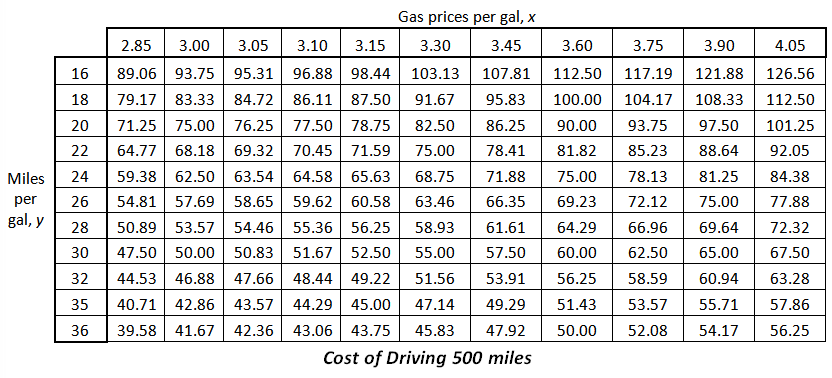
\includegraphics[height=0.27\textheight,keepaspectratio=1]{images/table.PNG}
    \end{figure}

    \begin{parts}
        \part If the cost, $C$, of driving 500 miles is given by $C(x,y)$ 
        according to the above table, find $C(3.60,26)$ and interpret it.
        \begin{subparts}
            \subpart Value: \answerline
            
            \subpart Interpretation: 

            \flexskip{1}

        \end{subparts} 
        \part Regular unleaded gasoline costs about \$3.85/gallon this week. 
        Find a formula for $C(3.85, y)$. Use your formula to plot this
        function in Sage. Write down the Sage command you used below.

        \flexskip{1}\vspace{6ex}

    \newpage

        \part Explain the significance of $C(x,26)$ in terms of 
        driving costs. Find a formula for $C(x,26)$.

        \flexskip{1}

        \part Use Sage to plot $C(x,26)$. Write the Sage command(s)
        you used below.
            
        \flexskip{1}

    \end{parts}

    \question Label the local extrema on the following contour plots. Say
    whether each extreme point is a maximum or a minimum.

    \begin{tikzpicture}
        \begin{axis}[view={0}{90}, axis lines=middle,
        xmin=-1, xmax=1,
        ymin=-1, ymax=1,
        zmin=-1, zmax=1,
        enlargelimits=false,
        xlabel=$x$, ylabel=$y$,
        plot box ratio=1,
        every node/.style = {circle, fill=black, thick, minimum size=1pt}]
        \addplot3[contour gnuplot={levels={-0.3,-0.2,-0.1,0,0.1,0.2,0.3}},thick,
        samples=100, 
        contour/draw color={black},
        contour/contour label style={nodes={text=black}}]
            {8*y^4+x^2+x*y-3*y^2-y^3};
        \end{axis}
    \end{tikzpicture} \hspace{1cm} 
    \begin{tikzpicture}
        \begin{axis}[view={0}{90}, axis lines=middle,
        xmin=-2, xmax=2,
        ymin=-2, ymax=2,
        zmin=-2, zmax=2,
        enlargelimits=false,
        xlabel=$x$, ylabel=$y$,
        plot box ratio=1,
        every node/.style = {circle, fill=black, thick, minimum size=1pt}]
        \addplot3[contour gnuplot={levels={-3,-2.5,-2,-1.5,-1,-0.5,0,0.5,1,1.5,2,2.5,3}},thick,
        samples=100, 
        contour/draw color={black},
        contour/contour label style={nodes={text=black}}]
            {x^3-x*y+y^3};
        \end{axis}
    \end{tikzpicture}

    \begin{tikzpicture}
        \begin{axis}[view={0}{90}, axis lines=middle,
        xmin=-1, xmax=1,
        ymin=-1, ymax=1,
        zmin=-0.5, zmax=0.5,
        enlargelimits=false,
        xlabel=$x$, ylabel=$y$,
        plot box ratio=1,
        every node/.style = {circle, fill=black, thick, minimum size=1pt}]
        \addplot3[contour gnuplot={levels={-2,-1.5,-1,-0.5,0,0.5,1,1.5,2}},thick,
        samples=80, 
        contour/draw color={black},
        contour/contour label style={nodes={text=black}}]
            {(x-y)*exp(x^2-y^2)};
        \end{axis}
    \end{tikzpicture} \hspace{1cm}
    \begin{tikzpicture}
        \begin{axis}[view={0}{90}, axis lines=middle,
        xmin=-1, xmax=1,
        ymin=-1, ymax=1,
        zmin=-0.5, zmax=0.5,
        enlargelimits=false,
        xlabel=$x$, ylabel=$y$,
        plot box ratio=1,
        every node/.style = {circle, fill=black, thick, minimum size=1pt}]
        \addplot3[contour gnuplot={levels={-4,-3,-2,-1,0,1,2,3,4}},thick,
        samples=80, 
        contour/draw color={black},
        contour/contour label style={nodes={text=black}}]
            {x^3+y^4-6*x-2*y^2};
        \end{axis}
    \end{tikzpicture}


\end{questions} 

\end{document}